\documentclass[titlepage]{article}
\usepackage{amsmath}
\usepackage{amsfonts}
\usepackage[T1]{fontenc}
\usepackage{tikz}
\usepackage{tikz-qtree}
\usepackage{forest}
\usepackage[style=numeric]{biblatex}
\usepackage{amsthm}
\usepackage{mathtools}
\usepackage{stmaryrd}
\usepackage{algorithm}
\usepackage{algpseudocode}
\usepackage{tabularx,ragged2e,booktabs,caption}
\usepackage{graphicx}



\addbibresource{refs.bib}
%\newtheoremstyle{break}{10pt}{0pt}{}{}{\bfseries}{}{\newline}{}
%\theoremstyle{break}
\newtheorem{theorem}{Theorem}
\newtheorem{lemma}{Lemma}
\newtheorem{definition}{Definition}
\newtheorem{example}{Example}
\newtheorem{proposition}{Porposition}

\newcommand*{\textcal}[1]{%
  % family qzc: Font TeX Gyre Chorus (package tgchorus)
  % family pzc: Font Zapf Chancery (package chancery)
  \textit{\fontfamily{qzc}\selectfont#1}%
}

%\newcommand{\Tmc}{\ensuremath{\mathcal{T}}\xspace}
\DeclareMathOperator{\st}{st}

\begin{document}
\section{Introduction}
Description Logics (DLs) are a family of formal logics designed for representing and inferring new
knowledge from defined knowledge encapsulated in ontologies. However, some ontologies like SNOMED or
LOINC \cite{article}
contain a vast number of axioms, making it challenging to extend them without generating unwanted 
inferences. Proofs, which are essentially trees consisting of axioms as vertices connected by 
direct consequence operators, can be useful in understanding the cause of these unwanted inferences. 
Recently, a new Java library called EVEE-LIBS \cite{https://doi.org/10.48550/arxiv.2206.07711} has been developed to generate proofs for DLs up to 
$\mathcal{ALCH}$. To achieve this, EVEE-LIBS uses Lethe \cite{KoopmannSchmidt15c}, a 
consequence-based reasoning procedure, to generate new axioms. However, the underlying direct 
consequence operator, which is Lethes underlying calculus, 
plays a critical role in determining the resulting proofs. Therefore, in this student project report, 
I will present an implementation of the alternative calculus proposed in [3] and compare the 
generated proofs to those of EVEE-LIBS. This comparison will provide valuable insights into the effectiveness of 
different calculi in generating proofs for ontologies, which could ultimately lead to improved 
methods for extending and reasoning about ontologies.



\section{The Description Logic $\mathcal{ALCH}$}
\begin{itemize}
  \item What is ALCH
  \item syntax and semantics
\end{itemize}

\subsection{Syntax}
The DL $\mathcal{ALCH}$ allows the operators concept negation ($\neg$), 
concept intersection ($\sqcap$), concept union ($\sqcup$), universal restriction
 ($\forall$), existential quantification ($\exists$), the top concept ($\top$),
 the bottom concept ($\bot$) and finally role hierarchies ($\sqsubseteq$).
With those operators and two additional sets of concept names ($N_C$) and role names ($N_R$),
one can then build all complex concepts of $\mathcal{ALCH}$ 
($N_{\mathcal{ALCH}}$) as follows:

    \begin{tabular}{l l}
      if $C \in N_C$ & then $C \in N_{\mathcal{ALCH}}$ \\
      if $C \in N_{\mathcal{ALCH}}$ & then $\neg C \in N_{\mathcal{ALCH}}$ \\
      if $C_1,C_2 \in N_{\mathcal{ALCH}}$ & then $C_1 \sqcap C_2 \in N_{\mathcal{ALCH}}$ \\
      if $C_1,C_2 \in N_{\mathcal{ALCH}}$ & then $C_1 \sqcup C_2 \in N_{\mathcal{ALCH}}$ \\
      if $C \in N_{\mathcal{ALCH}}$ and $r \in N_R$ & then $\exists r.C \in N_{\mathcal{ALCH}}$ \\
      if $C \in N_{\mathcal{ALCH}}$ and $r \in N_R$ & then $\forall r.C \in N_{\mathcal{ALCH}}$ \\
    \end{tabular} 

Now that complex concepts are defined we can also formalize the notion of a TBox.

\begin{definition}[TBox]
  A $\mathcal{ALCH}$ TBox $\mathcal{T}$ is a set of general concept inclusions and role inclusions i.e.
  $\mathcal{T} \subseteq \{C_1 \sqsubseteq C_2 \mid C_1, C_2 \in N_{\mathcal{ALCH}} \} \cup 
  \{r_1 \sqsubseteq r_2 \mid r_1, r_2 \in N_R\}$
\end{definition}

\begin{definition}[ABox]
  A ABox $\mathcal{A}$ is a set of concept and role assertions i.e.
  $\mathcal{A} \subseteq \{a:C \mid a \in N_I, C \in N_{\mathcal{ALCH}}\}
  \cup \{(a,b):r \mid a,b \in N_I, C \in N_{\mathcal{ALCH}}\}$
\end{definition}

\subsection{Semantics}
The semantics of the DL $\mathcal{ALCH}$ are defined by a first order logic interpretation
$I := (\Delta^I, \cdot^I)$, where $\Delta^I$ is the \emph{domain} of the interpretation
and $\cdot^I$ the interpretation function.
Concepts are then interpreted as follows:
\begin{definition}[Interpetation]
  Let $A \in N_C, C, D \in N_{\mathcal{ALCH}}, r \in N_R$ then
  \begin{center}
    \begin{tabular}{l c l}
      %use align* * := ohne nummerierung
    
      $\top^I$& $\coloneqq$& $\Delta^I$ \\
      $\bot^I$& $\coloneqq$& $\emptyset$\\      
      $A^I$ & $\coloneqq$ & $A'$ where $A' \subseteq \Delta^I$ \\
      $r^I$ & $\coloneqq$ & $R$ where $R \subseteq \Delta^I \times \Delta^I$\\
      $(\neg C)^I$ & $\coloneqq$ & $C^I$ \\
      $(C \sqcap D)^I$ & $\coloneqq$ & $C^I \cap D^I$ \\
      $(C \sqcup D)^I$ & $\coloneqq$ & $C^I \cup D^I$ \\
      $(\exists r.C)^I$ & $\coloneqq$ & $ \{a \in \Delta^I \mid \exists b \in \Delta^I : (a,b) \in r^I \text{ and } b \in C^I \}$ \\
      $(\forall r.C)^I$ & $\coloneqq$ & $ \{a \in \Delta^I \mid \forall b \in \Delta^I : (a,b) \in r^I \text{ then } b \in C^I \}$ \\
      \end{tabular}        
  \end{center}
\end{definition}  
This interpretation can then also be extended to GCIs and role inclusions. Since a GCI or role inclusions only hold
or not hold under a interpretation the holds operator ($\models$)is used to express this 
behaviour.

\begin{definition}
    For $C, D \in N_{\mathcal{ALCH}}: I \models C \sqsubseteq D  :\iff C^I \subseteq D^I$ \\
    For $r, s \in N_R: I \models r \sqsubseteq s  :\iff (\forall a,b \in \Delta^I: (a,b) \in r^I \Rightarrow (a,b) \in s^I$)
\end{definition}

\section{The Algorithm}
In this section I will describe how my Algorithm works and therefore start with what a
proof formally is.

\subsection{Proofs}
A proof is a list of GCIs $A_1, \ldots, A_n$, where for each $i \in \{1, \ldots n - 1\}
$ $\{A_1, \ldots, A_i\} \models A_{i+1}$. Since my approach uses rules to derive such
proofs I now define a rule based definition of a proof. A rule based proof is not a list
of GCIs but rather a list of inferences, where a inference is a tuple $((\phi_1, \ldots, \phi_n), \psi, \mathbf{R})$,
where $\phi_1, \ldots, \phi_n,$ are GCIs and the list containing them is called premise, $\psi$ is also a GCI
and called the conclusion and $\mathbf{R}$ is a rule. In order a list of inferences
to be a proof it has to hold that for all inferences the premise and conclusion actually have to be an 
instance of $\mathbf{R}$.

\subsection{Normalization}\label{alg:norm}
Before we dive into the rule based procedure, we first need to be sure, that our ontology has the right form.
\begin{definition}[Normalform]
  An ontology $\mathcal{O}$ is said to be in normalform iff all axioms in $\mathcal{O}$ are of the form
  $\bigsqcap A_i \sqsubseteq \bigsqcup B_j, A \sqsubseteq \exists r.B, \exists r.A \sqsubseteq A, A \sqsubseteq \forall r.B$ 
  or $r \sqsubseteq s$, where $A_i, B_j, A, B $ are concept names and $r,s$ are role names.
\end{definition}
An $\mathcal{ALCH}$ ontology $\mathcal{O}$ can then be easily transformed into this normalform by first 
using the
\emph{structural transformation} $\st: N_C \rightarrow N_C$. $\st$ is defined as follows:

\begin{center}

\begin{tabular}{c c }
$\st(A) \coloneqq  A$ & $\st(C \sqcap D) \coloneqq  [C]$\\
$\st(\top) \coloneqq \top$ & $\st(C \sqcup D) \coloneqq [C] \sqcup [D]$ \\
$\st(\bot) \coloneqq \top$ & $\st(\exists r.C) \coloneqq [C] \exists r.[C]$\\
$\st(\neg C) \coloneqq \neg [C]$ & $\st(\exists r.C) \coloneqq [C] \exists r.[C]$\\
\end{tabular}
\end{center}
where for a concept $C$ [C] is just a new atom that corresponds to $C$.
Now we obtain a new structual transformed ontology $\st(\mathcal{O})$ form $\mathcal{O}$ by
first adding all role inclusions or $\mathcal{O}$ into it and then adding 
\begin{itemize}
  \item $\st(C) \sqsubseteq [C]$ for every negative $ C \in \mathcal{O}$ 
  \item $[D]\sqsubseteq \st(D)$ for every positive $D \in \mathcal{O}$
  \item $[C] \sqsubseteq [D]$ for every axiom $C \sqsubset D$ occuring $C \in \mathcal{O}$
\end{itemize}

$\st(\mathcal{O})$ needs then to be further normalized by removing all axioms of the form $\forall r.C \sqsubseteq A$ and
adding $\neg \exists r. \neg C $. Note that both axioms are actually equivalent.
Finally the following normalization rules have to be applied to $\st(\mathcal{O})$ until no rule can be applied
anymore.

  \begin{itemize}
    \item $ \dfrac{[C \sqcap D] \sqsubseteq [C] \sqcap [D]}{ [C \sqcap D] \sqsubseteq [C], \quad [C \sqcap D] \sqsubseteq [D]}$
    \item $ \dfrac{[C] \sqcup [D] \sqsubseteq [C \sqcap D]}{ [C] \sqsubseteq [C \sqcup D], \quad [D] \sqsubseteq [C \sqcup D]}$
    \item $ \dfrac{[\neg C] \sqsubseteq \neg [C] }{ [\neg C ] \sqcap [C] \sqsubseteq \bot}$
    \item $ \dfrac{\neg [C] \sqsubseteq [\neg C] }{ \top \sqsubseteq [\neg C ] \sqcap [C]}$
  \end{itemize}

\subsection{Inference rules}
\begin{definition}[Inference Rules]
  
\end{definition}
On a normalized ontology we can now apply the following inference rules.



\begin{align}
  \mathbf{R^{+}_A} & \dfrac{}{H\sqsubseteq A} : A \in H \label{rules:RPlusA}\\
  \mathbf{R^{-}_A} & \dfrac{H \sqsubseteq N \sqcup A}{H \sqsubseteq N} : \neg A \in H  \label{rules:RMinusA}\\ 
  \mathbf{R^{n}_{\sqcap}} & \dfrac{\{H \sqsubseteq N_i \sqcup A_i \}^{n}_{i=1}}{H \sqsubseteq \bigsqcup^{n}_{i=1} N_i \sqcup M} : \bigsqcap^{n}_{i=1} A_i \sqsubseteq M \in \mathcal{O} \label{rules:RNAnd} \\
  \mathbf{R^+_{\exists}} & \dfrac{H \sqsubseteq N \sqcup A }{ H \sqsubseteq N \sqcup \exists r.B} : A \sqsubseteq \exists r.B \in \mathcal{O} \label{rules:RPlusExists}\\
  \mathbf{R^-_{\exists}} & \dfrac{H \sqsubseteq M \sqcup \exists r.K,\quad K \sqsubseteq N \sqcup A}{H \sqsubseteq M \sqcup B \sqcup \exists r.(K \sqcap \neg A)} : \exists s.A \sqsubseteq B \in \mathcal{O} \quad r \sqsubseteq_{\mathcal{O}} s \label{rules:RMinusExists}\\
  \mathbf{R^\bot_{\exists}} & \dfrac{H \sqsubseteq M \sqcup \exists r.K,\quad K \sqsubseteq \bot}{H \sqsubseteq M} \label{rules:RBotExists}\\
  \mathbf{R_{\forall}} & \dfrac{H \sqsubseteq M \sqcup \exists r.K,\quad H \sqsubseteq N \sqcup A}{H \sqsubseteq M \sqcup N \sqcup \exists r.(K \sqcap B)} : A \sqsubseteq \forall s.B \in \mathcal{O} \quad r \sqsubseteq_{\mathcal{O}} s \label{rules:RForall}
\end{align}



where $M,N$ are disjunctions of atoms and $H,K$ are conjunctions of literals.

\begin{algorithm}
  \caption{Main Loop}\label{alg:cap}
\begin{algorithmic}
  \Procedure{main}{ontology, goal}
  \State Normalizer.normalize(ontology)

  \State proofHandler $\gets$ new ProofHandler(query)
  \State rules $\gets$ getRules(ontology, proofHandler) 
  \While{notFinished(proofHandler)} 
  \For{(rule in rules)}
    \State setNewRule(rule.apply())
  \EndFor
  \EndWhile
  \EndProcedure
\end{algorithmic}
\end{algorithm}


The algorithms main loop consists of two stages: normalization and rule application.
The normalization stage implements the algorithm as outlined in section \ref{alg:norm}. The normalized
ontology and a new instance of a ProofHandler are then used to create instances of each rule type. 
Every rule, except for \ref{rules:RPlusA}, \ref{rules:RMinusA} and \ref{rules:RBotExists}   which do not need ontology axioms, need these two as 
arguments. The ontology is preprocessed, such that all relevant ontology axioms are saved in a way which 
allows for an easier rule application and prevents searching for relevant axioms every time the rule is 
applied. The ProofHandler provides active axioms from which rules are able to create new axioms and processes
them, as described in \ref{alg:proofHandler}, to generate new inferences. The created rules are then applied 
one after each other until the halting condition is met.  The halting condition is set to true either when 
the goal concept is reached or when all rules are unable to generate a new axiom in an iteration. 


\subsection{Proof Handler}\label{alg:proofHandler}
The ProofHandler is the main component of the algorithm. It is responsible for handling new produced axioms,
provides the rules with these new axioms, checks whether the halting condition is met and creates a proof
in case the algorithm finds one. The ProofHandler is initialized with the query axiom. The sub concept of this
axiom is added to the list of active axioms and the super concept is saved in order to check whether the goal
was found. The handling of newly produced axioms contains the following steps. First the ProofHandler is provided
with all axioms which were used to generate, the new axiom the newly generated axiom and the name of the rule which 
calls the method. In case of rules which also use ontology axioms
the provided axioms are split into premises and ontology premises. This information is then used to create a new
Inference and add the new axiom to the list of active Axioms. Since some rules do generate some axioms multiple
times the ProofHandler also checks whether the axiom is already in the list of active axioms and depending on
the outcome of this check returns the information whether a new Inference was created. While doing so it is also
checked whether the super concept of the new axiom is the goal axiom. In case the algorithm stops
and the goal was found the ProofHandler also provides a method to create a proof. In order to prevent to just
return all Inferences which were created during the algorithm the ProofHandler uses the Java library EVEE to create
a meaningful proof.
EVEE not only provides data structures like Inferences and Proofs but also has different algorithms to create
different types of proofs. In this project I use the algorithm which creates a proof with the lowest depth possible.


\subsection{Inference Rules}\label{alg:rules}
In this subsection I will describe how each inference rule is implemented and what data structures they use.
%ITS IMPORTANT TO FLATTEN CONCEPTS
% and empty conjunctions and conjunctions with only one element !!!!!

%In this subsection I will describe how the inference rules are implemented. Let's start
%which inputs and output types of each rule implementation. Most rule implementations
% need two kinds of resources. Axioms which are part of the given ontology and axioms, which are
%active. An axiom is said to be active if it was previously created by some rule. This is 
%not the case for rule \ref{rules:RPlusA}, \ref{rules:RMinusA} and \ref{rules:RBotExists}. Instead, the rules \ref{rules:RPlusA} and \ref{rules:RMinusA} use active concepts to
%produce new axioms, where active concepts, similar to active axioms, are concepts, which
%were created by some rule. The rule (1) does not even use any active axioms. And all rules
%have in common, that they produce on each application, but it is not so simple for the 
%rule implementations. Due to the matching process most rules produce in one application
%more than one axiom. Now I will go over every rule in more detail and will describe of 
%they were implemented
\subsubsection{The rule $\mathbf{R^{+}_A}$}
The rule \ref{rules:RPlusA} is one of the simplest rules, since it does not use any active axioms and
also no axioms from the ontology. The only thing that has to be taken care of is
creating new axioms from active concepts. In order to do that the implementation iterates
through all active concepts and searches for conjunctions or atoms, which are seen as conjunctions of size 1.
In case a conjunction is found all atoms within the conjunction are saved to a list.
Each element is then used as super concept of a new axiom with its origin axiom as sub concept.
After the handling of all active concepts the implementation empties the list of active concepts in order to
reduce redundant axiom creation.

\subsubsection{The rule $\mathbf{R^{-}_A}$}
This rule also does not use any axioms from the ontology but does use active axioms.
The implementation, first searches for axioms with a conjunction as sub concept, which contain negative
literals. In case such an axiom was found the implementation searches for a positive literal in the super concept
of the axiom. If the super concept contains the positive literal the implementation creates a new axiom with 
the same sub concept as the origin axiom and the super concept of the origin axiom without the positive literal.
Note that used active axioms are not removed from the list of active axioms, which allows the possibility of
redundant axiom creation. In order to tackle this problem I created an alternative rule implementation
which checks before handling an active axiom
whether it was already used by this rule. To achieve this the rule stores all used axioms in a set. This set can 
become very large and in worst case can contain all active axioms. That's why I made it an alternative implementation
in order to allow for a time optimized version of the algorithm and a space optimized version of the algorithm.

\subsubsection{The rule $\mathbf{R^{n}_{\sqcap}}$}

The rule \ref{rules:RNAnd} is the first rule which uses axioms from the ontology.
On creation of its implementation first the ontology
gets filtered for axioms of the form $\bigsqcap^{n}_{i=1} A_i \sqsubseteq M$
These axioms get saved into a list of tuples where the first element of the tuple is the conjunction
stored as a set and the second element is the entire axiom, which will not only be used to get its super concept
for creation of a new axiom but also in order to pass it as ontology premise to the ProofHandler.

On application of the rule the following 
function $m  \coloneqq N_{\mathcal{ALCH}} \times N_C \rightarrow \{N \mid N \subseteq N_C\}$
is defined by using the current active axioms. First all active axioms get filtered for
axioms of the form $H \sqsubseteq N \sqcup A$, where $H$ is conjunctions of literals $N$ disjunctions
 of atoms and $A$ an atom. Every axiom is then used to define the function m in the following way:
 For each active axiom $\alpha = H \sqsubseteq N \sqcup A: m(H,A) \coloneqq \{N_c | N_c \in N\}$.
 After the function is defined it will be used to compose derived axioms.
 In order to do so the implementation first iterates through all ontology axioms and checks,
 whether the LHS of a given axiom is subsumed by the right entry of the domain of m. If this is
 the case, m can be used to find for all $A_i$ in the matched ontology axiom the corresponding
 $N_i$ and in the end the new axiom $H \sqsubseteq \bigsqcup^{n}_{i=1} N_i \sqcup M$ is created.



When the rule is applied to the set of active axioms the rule first maps all axioms
with an equal subconcept to a tuple, where the first entry is a list of concept names,
which where these concept names corresponds to all $A_i$ which can be found for a given
subconcept $H$ and the second entry is a map which maps a concept name which 
is a particular $A_i$ and maps it to a tuple where its first entry is a list of all concept 
names in the corresponding $N_i$ and the second entry is just the hole axiom 
$H \sqsubseteq N_i \sqcup A_i$. 

After the map is created the rule starts to iterate 
through the ontology axioms and the created entries of the just created map and looks for
entries in the map where the set of $A_i$s from the list, which was created from the ontology,
is subsumed by some set in the set in first entry of the map.
When such a match was found we have all need elements to create the new axiom 
$H \sqsubseteq \bigsqcup^{n}_{i=1} N_i \sqcup M$ in order to get all requiered $N_i$s
the list of $A_i$s of the ontology axiom is used to filter the map in the second entry
of the entry of the just created map.

\subsubsection{The rule $\mathbf{R^+_{\exists}}$}
The rule (4) is also uses axioms from the ontology so on creation of the rule
 implementation the ontology gets filtered for axioms of the form 
 $A \sqsubseteq \exists r.B \in \mathcal{O}$. When the rule implementation is applied,
 the active axioms just get filtered for 

 \subsubsection{The rule $\mathbf{R^-_{\exists}}$}
The rule (5) not only uses axioms from the ontology but also uses role inclusions, which
follow from the ontology. The role inclusions are calculated separately since rule (7) 
also uses them. So the only thing that has to be done on creation is, that axioms of the form
$\exists s.A \sqsubseteq B$ need to be filtered.
On rule application the rule implementation then first filters the active axioms for
axioms where the superconcept is a disjunction of concept names and one of them matches
some $A$ in some ontology axiom. The matched axioms then are mapped to their subconcepts $K$.
After this is done the just created map is used to find axioms of the form 
$H \sqsubseteq M \sqcup \exists r.K$

\subsubsection{The rule $\mathbf{R^\bot_{\exists}}$}
The rule (6) does not use no axioms from the original ontology. Usually there are way more axioms 
containing existential restrictions than axioms with the bottom concept on the right hand side and
therefore the implementation first filters for axioms of the form $K \sqsubseteq \bot$ safes them
in a list $l$. Afterwards
the rule implementation filters for rules of the form $H \sqsubseteq M \sqcup \exists r.K $
and checks if a axiom of this form is found, if the K already occures in some LHS of an axiom in
$l$. From this found rule then the new axiom $H \sqsubseteq M$ can then be created immediately.

\subsubsection{The rule $\mathbf{R_{\forall}}$}
The rule (7) is no the final rule now again uses from the ontology following role inclusions
and also axioms from the ontology of the form $A \sqsubseteq \forall s.B$. Therefore, on 
creation of the rule implementation first the ontology gets filtered for such axioms, where 
the role s is on the right hand side of some implied role inclusion.
On application of the rule implementation first searches for active axioms of the form
$H \sqsubseteq M \sqcup \exists r.K$ where r has to match some RHS of some matched role inclusion.
The found axioms are then used to define a function $m_l \coloneqq N_ \rightarrow$


\begin{example}
  Let $\mathcal{O} = \{ B \sqsubseteq \exists r.D, A \sqsubseteq \forall s.E, \exists r.E \sqsubseteq C, r \sqsubseteq s\}$
  then a proof for $A \sqcap B \sqsubseteq C $ would look like the following: \\
    $(((),A \sqcap B \sqsubseteq B, \mathbf{R^+_A}),$ \\
    $((A \sqcap B \sqsubseteq B, B \sqsubseteq \exists r.D), A \sqcap B \sqsubseteq \exists r.D, \mathbf{R^+_{\exists}}), $ \\
    $((A \sqcap B \sqsubseteq \exists r.D, A \sqsubseteq \forall s.E, r \sqsubseteq s),A \sqcap B \sqsubseteq \exists r.(D \sqcap E), \mathbf{R_{\forall}}), $ \\
    $((),(D \sqcap E) \sqsubseteq E, \mathbf{R^+_A}),$ \\
    $((A \sqcap B \sqsubseteq \exists r.(D \sqcap E), (D \sqcap E) \sqsubseteq E, \exists r.E \sqsubseteq C), A \sqcap B \sqsubseteq \exists r.(D \sqcap E \sqcap \neg E) \sqcup C, \mathbf{R^-_{\exists}}),$ \\
    $((), D \sqcap E \sqcap \neg E \sqsubseteq E, \mathbf{R^+_A}), $ \\
    $((D \sqcap E \sqcap \neg E \sqsubseteq E),D \sqcap E \sqcap \neg E \sqsubseteq \bot, \mathbf{R^-_A}),$ \\
    $((A \sqcap B \sqsubseteq \exists r.(D \sqcap E \sqcap \neg E) \sqcup C, D \sqcap E \sqcap \neg E \sqsubseteq \bot), A \sqcap B \sqsubseteq C, \mathbf{R^{\bot}_{\exists}}))$
\end{example}
Notes that in the algorithm not only these concepts would be created but also other rules.
For example even in the first step not only $A \sqcap B \sqsubseteq B$ would have been created but also
$A \sqcap B \sqsubseteq A$.



\subsection{Problems}
While implementing the algorithm I encountered some problems, which I will discuss in the following.

\begin{itemize}
  \item no nested conjunctions
\end{itemize}

WHY DOES MY APPROACH WORK


\begin{itemize}

  \item proofs definition
  \item calcül
  \item example 
  \item pseudo code
  \item normalform
  \item normalization
  \item rule application
  \item probleme discutieren !!!!
\end{itemize}

\section{Proof Generation}
\begin{figure}
  \centering
  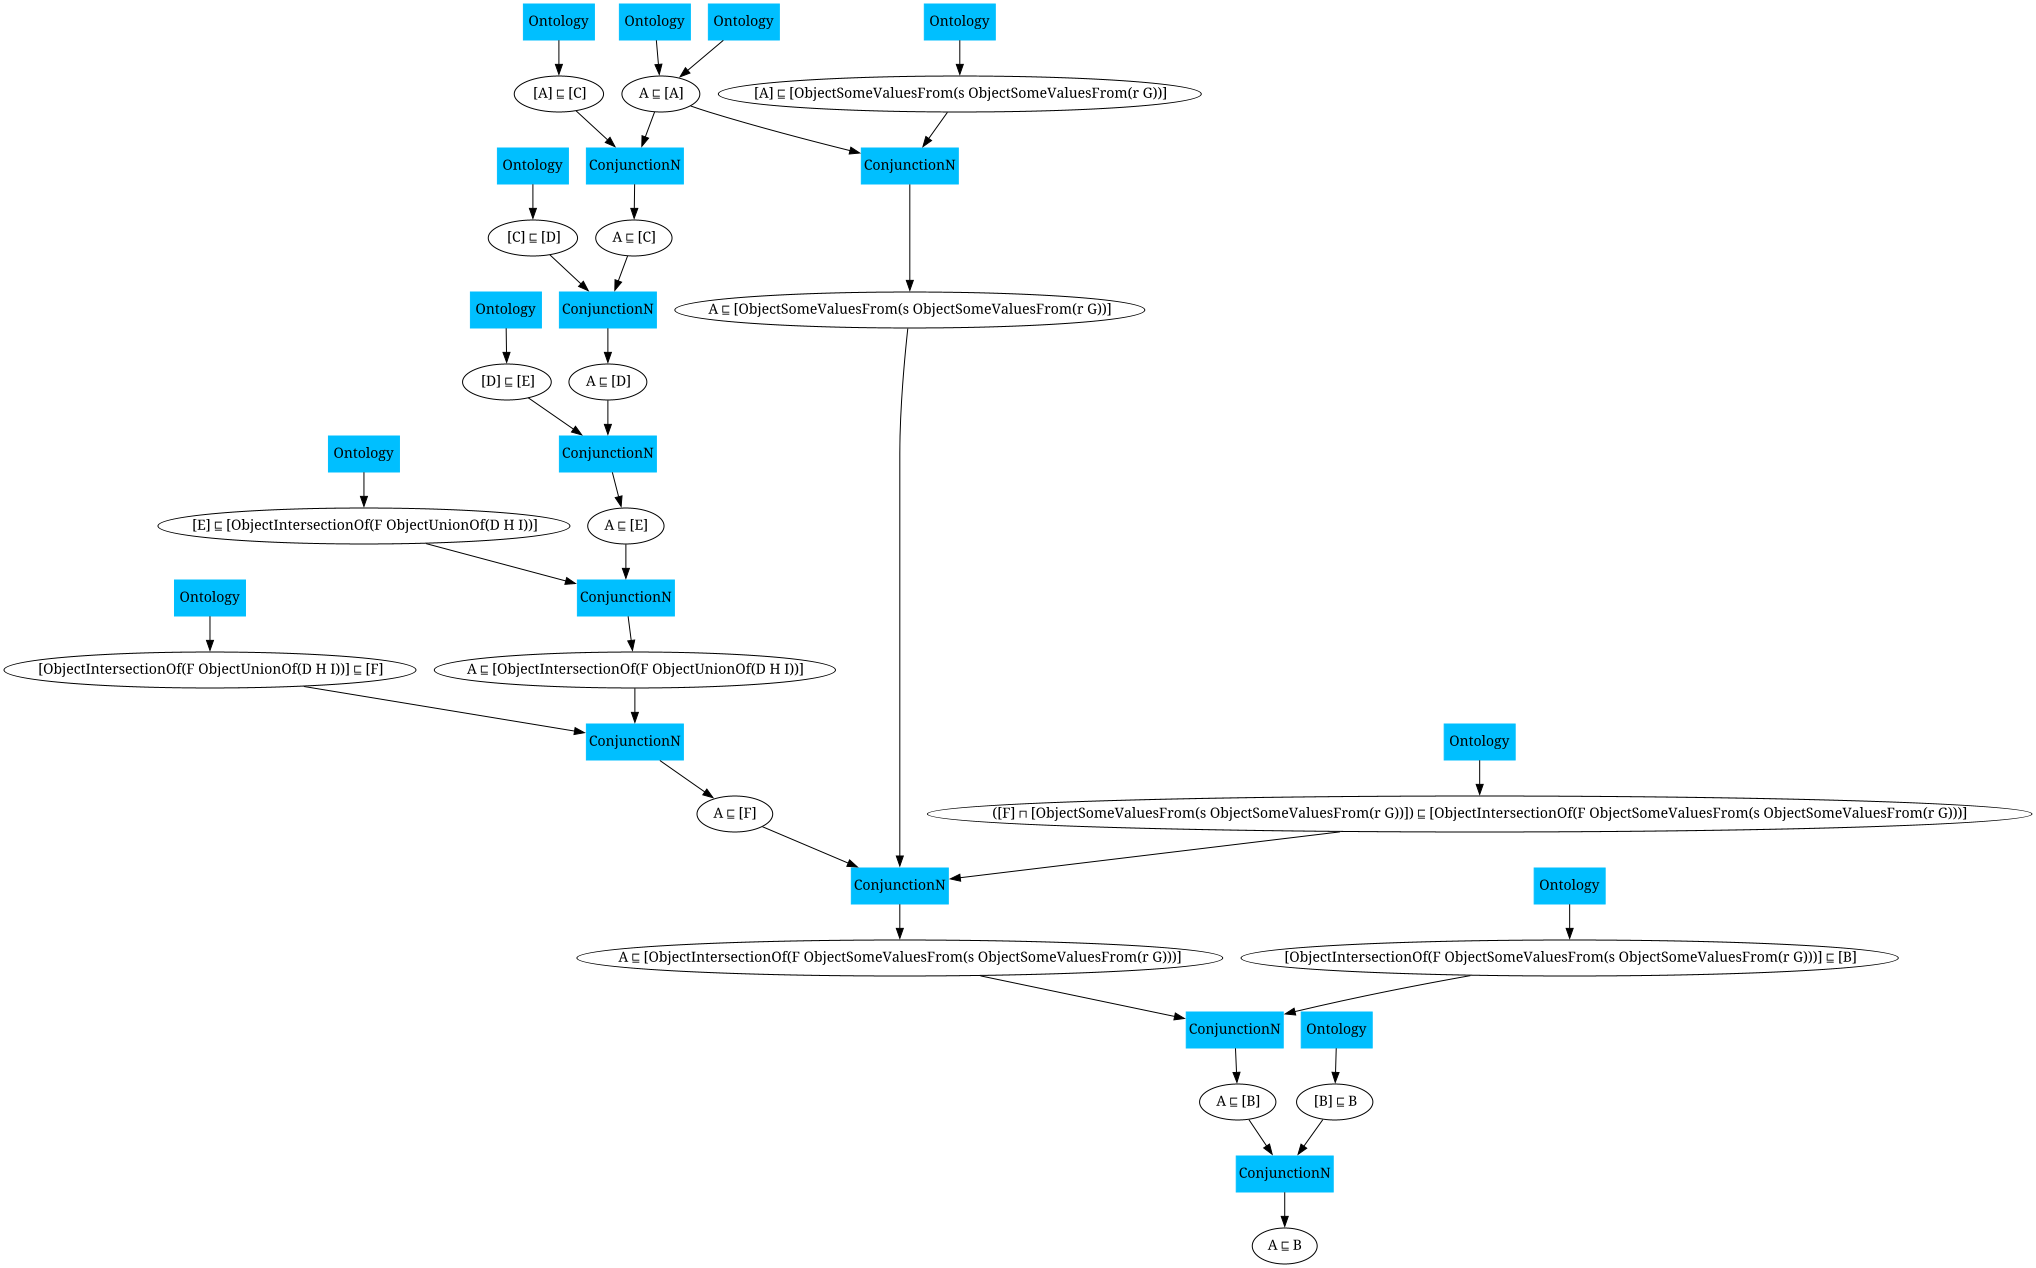
\includegraphics[width=1\textwidth]{pictures/ALCH_task00001.png}
  \caption{ALCH-Reasoner Proof for Task 1}
  \label{fig:label}
\end{figure}


\begin{figure}
  \centering
  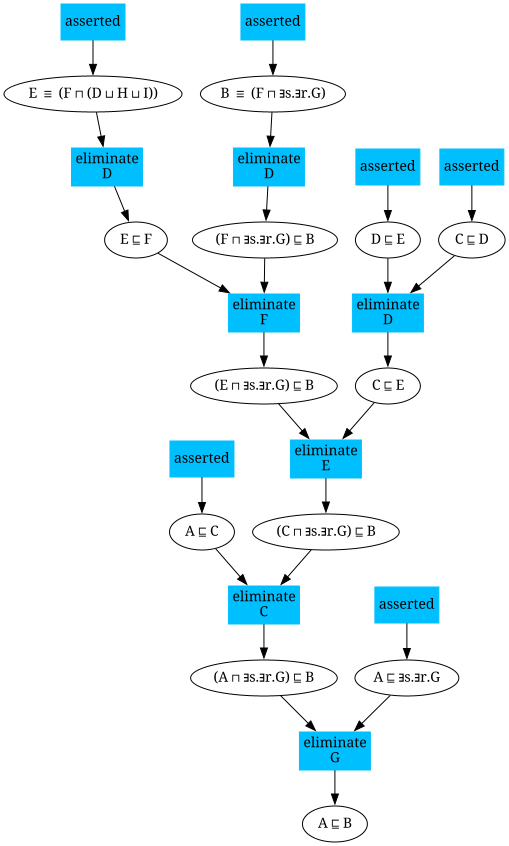
\includegraphics[width=1\textwidth]{pictures/Lethe_task00001.png}
  \caption{Lethe Proof for Task 1}
  \label{fig:label}
\end{figure}

When comparing the proofs generated by the ALCH-Reasoner and the Lethe-Reasoner, one can see that the 
proofs differ quite substantially. While for example the ALCH-Reasoner uses only the $mathbf{R^{n}_{\sqcap}}$ rule
on a normalized task 1 ontology, the Lethe-Reasoner only uses quite a few different types of elimination rules. 



Nicht zwingened notwendig
\begin{itemize}
  \item UML diagrams
  \item normalization
  \item inference rules
  \item loop
  \item proof building
  \item export
\end{itemize}
\section{Results}
\begin{itemize}
  \item test on Pizza
  \item nice diagrams
\end{itemize}

proof generator main task file 

\printbibliography
\end{document} 
